\chapter{Introduction}

The \textit{Sawyer: Peg in a hole} challenge is used to get an introduction
into the field of robotics and the robot Sawyer.

\begin{figure}[H]
	\begin{center}
		
\includegraphics[width=0.3\linewidth]{images/ostfalia_logo_left.png}
		\caption{TODO: Add Picture}
	\end{center}
\end{figure}

The behavior of \textbf{Sawyer} in this challenge shall be programmed by using the own toolchain called \textbf{Intera}.
Intera is a block orientated programming system that controls the robot by changing the robots pose
with poses that were defined in the programming step.
The robot can changes poses relatively to the previous pose.

\section{Task description: Basic}

The robot shall pickup a pin from a hole and move it to a different.
The so called \textit{PegBoard} has different type of holes.
For two holes the pin fits perfectly,
for two holes the pin fits loosely and
two dont fit at all.

\begin{figure}[H]
	\begin{center}
		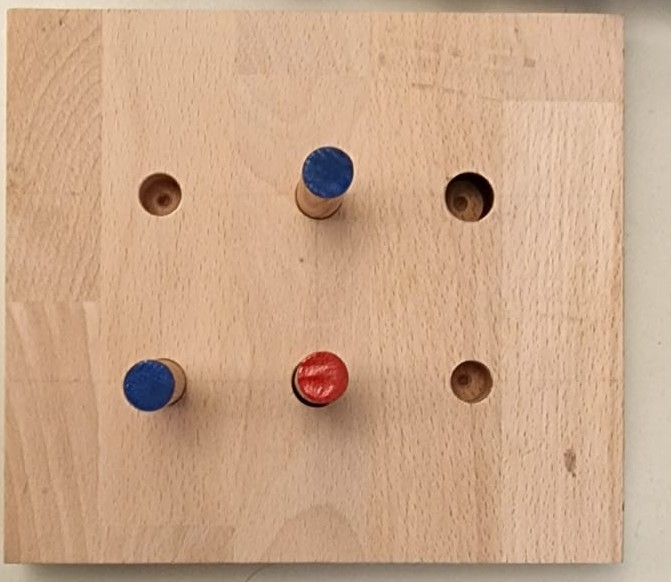
\includegraphics[width=0.3\linewidth]{images/PegBoard.png}
		\caption{TODO: Add Picture}
	\end{center}
\end{figure}

\section{Task description: Advance}

Based on the basic task, the advanced task is to play on a round board.

\begin{figure}[H]
	\begin{center}
		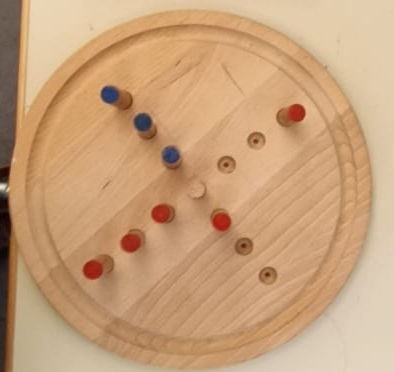
\includegraphics[width=0.3\linewidth]{images/PegBoardRound.png}
		\caption{TODO: Add Picture}
	\end{center}
\end{figure}

The challenge here is that the pins need to be moved over each other one after another in order to reach the other side.
